\documentclass[11pt,a4paper]{article}

% ---------- Packages ----------
\usepackage[margin=1in]{geometry}
\usepackage{graphicx}
\usepackage{booktabs}
\usepackage{xcolor}
\usepackage{hyperref}
\usepackage{xurl}
\usepackage{caption}
\usepackage{fancyhdr}
\usepackage{listings}
\usepackage{amsmath}
\usepackage{float}
\usepackage{enumitem}
\usepackage{titlesec}
\usepackage{array}

% ---------- Colors ----------
\definecolor{codebg}{RGB}{245,245,245}
\definecolor{codekeyword}{RGB}{0,0,180}
\definecolor{codecomment}{RGB}{0,130,0}
\definecolor{codestring}{RGB}{160,0,0}
\definecolor{headercolor}{RGB}{30,30,90}

% ---------- Hyperref ----------
\hypersetup{
    colorlinks=true,
    linkcolor=blue,
    urlcolor=blue,
    citecolor=blue,
    pdftitle={CNN Image Classification - Rock Paper Scissors Lab Report},
    pdfauthor={Shafikul Islam Marwan}
}

% ---------- Code listing style ----------
\lstdefinestyle{pythonstyle}{
    backgroundcolor=\color{codebg},
    commentstyle=\color{codecomment},
    keywordstyle=\color{codekeyword}\bfseries,
    stringstyle=\color{codestring},
    basicstyle=\ttfamily\small,
    breaklines=true,
    breakatwhitespace=false,
    captionpos=b,
    keepspaces=true,
    numbers=left,
    numbersep=6pt,
    numberstyle=\tiny\color{gray},
    showspaces=false,
    showstringspaces=false,
    showtabs=false,
    tabsize=4,
    frame=single,
    rulecolor=\color{gray!40},
    language=Python
}
\lstset{style=pythonstyle}

% ---------- Section styling ----------
\titleformat{\section}{\normalfont\Large\bfseries\color{headercolor}}{\thesection}{1em}{}
\titleformat{\subsection}{\normalfont\large\bfseries\color{headercolor}}{\thesubsection}{1em}{}

% ---------- Header/Footer ----------
\setlength{\headheight}{14pt}
\pagestyle{fancy}
\fancyhf{}
\fancyhead[L]{CNN Image Classification -- Rock Paper Scissors}
\fancyhead[R]{ID: 220121}
\fancyfoot[C]{\thepage}
\renewcommand{\headrulewidth}{0.4pt}

\setlength{\parskip}{0.5em}
\setlength{\parindent}{0pt}

\begin{document}

% ==================================================
% TITLE PAGE
% ==================================================
\begin{titlepage}
    \thispagestyle{empty}
    \vspace*{0.2cm}

    \noindent
    \begin{minipage}[c]{0.16\textwidth}
        
\includegraphics[height=2.3cm]{images/just_logo.jpg}
    \end{minipage}%
    \begin{minipage}[c]{0.82\textwidth}
        \raggedright
        {\Large \textbf{Department of Computer Science and Engineering}}
    \end{minipage}

    \vspace{0.2cm}
    \rule{\linewidth}{0.8pt}

    \vspace{0.5cm}
    \begin{center}
        {\LARGE \textbf{Jashore University of Science and Technology}}\\[0.2cm]
        {\normalsize Faculty of Engineering and Technology - FET}
    \end{center}

    \vspace{2.2cm}
    \begin{center}
        {\Large \textbf{Lab Report}}\\[0.35cm]
        {\Large \textbf{On}}\\[0.35cm]
        {\Large \textbf{CNN Image Classification with PyTorch}}
    \end{center}

    \vspace{2cm}
    \begin{center}
        \textbf{Date of submission: 17 August 2026}
    \end{center}

    \vspace{2.8cm}

    \begin{center}
    \setlength{\fboxsep}{16pt}
    \fbox{
    \begin{minipage}{0.92\textwidth}
        \begin{minipage}[t]{0.46\textwidth}
            \raggedright
            \underline{\textbf{Submitted To:}}\\[10pt]
            \textbf{Instructor: Dr.\ A F M Shahab} \\ \textbf{Uddin}\\
            \textbf{Assistant Professor}\\
            \textbf{Department of CSE, JUST}\\
            \textbf{Course Title: Artificial} \\ \textbf{Intelligence and Machine Learning Lab}\\
            \textbf{Course Code: CSE 3202}
        \end{minipage}%
        \hfill
        \vrule width 0.6pt
        \hfill
        \begin{minipage}[t]{0.46\textwidth}
            \raggedright
            \underline{\textbf{Submitted By:}}\\[10pt]
            \textbf{Name: Shafikul Islam Marwan}\\
            \textbf{Student ID: 220121}\\
            \textbf{Registration Number: 2201020}\\
            \textbf{Year: 3\textsuperscript{rd}}\\
            \textbf{Semester: 2\textsuperscript{nd}}
        \end{minipage}
    \end{minipage}
    }
    \end{center}

    \vfill

\end{titlepage}

% ==================================================
% TABLE OF CONTENTS
% ==================================================
\tableofcontents
\newpage

% ==================================================
% 1. INTRODUCTION
% ==================================================
\section{Introduction}

Convolutional Neural Networks (CNNs) are the standard deep learning architecture for image classification tasks because they exploit spatial locality and translation invariance through learned convolutional filters. This lab implements a complete CNN classification pipeline in PyTorch that bridges standard benchmark-dataset training with real-world testing, as required by the assignment brief (\textit{Assignment: CNN Image Classification with PyTorch}).

The chosen task is \textbf{Option 2: Hand Gestures (Rock--Paper--Scissors)}. A CNN is trained from scratch on the publicly available Rock--Paper--Scissors (RPS) dataset created by Laurence Moroney, and is then evaluated on 10 custom photographs of the author's own hand captured with a smartphone camera, showing the Rock, Paper, and Scissors gestures.

\subsection{Objectives}
\begin{itemize}[leftmargin=1.3cm]
    \item Build a full CNN training/evaluation pipeline in PyTorch, automated end-to-end in Google Colab.
    \item Automatically retrieve the standard RPS dataset (via direct download) and custom phone images (via \texttt{git clone} of a GitHub repository) with no manual uploads.
    \item Design, train, and evaluate a CNN classifier on the standard dataset.
    \item Test the trained model on real-world smartphone photographs and critically analyze the results.
    \item Visualize training curves, a confusion matrix, misclassified samples, and a custom-image prediction gallery.
\end{itemize}

% ==================================================
% 2. DATASET
% ==================================================
\section{Dataset Description}

\subsection{Standard Dataset -- Rock, Paper, Scissors}
The model is trained on the well-known synthetic Rock--Paper--Scissors dataset released by Laurence Moroney, downloaded automatically inside the notebook from:
\begin{itemize}[leftmargin=1.3cm]
    \item Training set: \url{https://storage.googleapis.com/download.tensorflow.org/data/rps.zip}
    \item Test set: \url{https://storage.googleapis.com/download.tensorflow.org/data/rps-test-set.zip}
\end{itemize}

The dataset contains CGI-rendered images of hands making the three gestures against a plain background, at varying angles, skin tones, and lighting. The class distribution is perfectly balanced, as shown in Table~\ref{tab:dataset}.

\begin{table}[H]
\centering
\caption{Rock--Paper--Scissors dataset split summary}
\label{tab:dataset}
\begin{tabular}{lccc}
\toprule
\textbf{Split} & \textbf{Paper} & \textbf{Rock} & \textbf{Scissors} \\
\midrule
Training & 840 & 840 & 840 \\
Test & 124 & 124 & 124 \\
\midrule
\textbf{Total} & 964 & 964 & 964 \\
\bottomrule
\end{tabular}
\end{table}

In total there are \textbf{2,520 training images} and \textbf{372 test images} across the three balanced classes: \texttt{paper}, \texttt{rock}, \texttt{scissors}.

\begin{figure}[H]
    \centering
    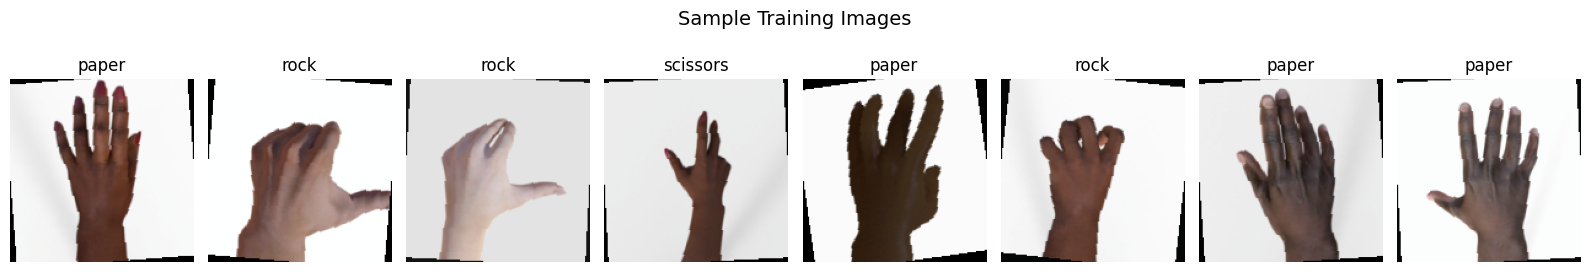
\includegraphics[width=0.95\textwidth]{images/sample_training_images.png}
    \caption{Sample images from the RPS training set, one batch drawn at random with augmentation applied.}
    \label{fig:sample_training}
\end{figure}

\subsection{Custom Real-World Dataset}
To evaluate real-world generalization, 10 original smartphone photographs were taken of a human hand performing the three gestures against a plain wall background: 3 images of \texttt{paper}, 4 images of \texttt{rock}, and 3 images of \texttt{scissors}. These images were committed to the \texttt{dataset/} folder of the GitHub repository and are cloned automatically at runtime -- no manual upload is required.

% ==================================================
% 3. METHODOLOGY
% ==================================================
\section{Methodology}

\subsection{Pipeline Overview}
The entire workflow is automated inside a single Colab notebook (\texttt{220121.ipynb}) and executes without any manual intervention, satisfying the assignment's reproducibility requirement:
\begin{enumerate}[leftmargin=1.3cm]
    \item Clone the GitHub repository with \texttt{!git clone} to obtain the 10 custom phone images.
    \item Download and extract the standard RPS train/test archives with \texttt{requests} and \texttt{zipfile}.
    \item Build \texttt{torchvision.transforms} pipelines and \texttt{DataLoader} objects.
    \item Define the CNN architecture as an \texttt{nn.Module} subclass.
    \item Train for 10 epochs, tracking loss/accuracy history.
    \item Save the trained weights as \texttt{220121.pth} (both locally and into the cloned repo's \texttt{model/} folder).
    \item Generate training curves, a confusion matrix, and visual error analysis on the standard test set.
    \item Run inference on the 10 custom phone images and display a prediction gallery.
\end{enumerate}

\subsection{Data Preprocessing}
All images are resized to $150\times150$ pixels and normalized using ImageNet mean/std statistics, so that the pretrained-style normalization is consistent across both the standard dataset and the custom phone photos. For the training split, additional data augmentation is applied to improve generalization; the test/validation split uses only deterministic resizing and normalization.

\begin{table}[H]
\centering
\caption{Preprocessing / augmentation pipeline}
\label{tab:transforms}
\begin{tabular}{ll}
\toprule
\textbf{Stage} & \textbf{Transform} \\
\midrule
Training & Resize(150,150) \\
 & RandomHorizontalFlip($p=0.5$) \\
 & RandomRotation($\pm10^{\circ}$) \\
 & ColorJitter(brightness=0.1, contrast=0.1) \\
 & ToTensor() \\
 & Normalize(mean=[0.485, 0.456, 0.406], std=[0.229, 0.224, 0.225]) \\
\midrule
Test / Custom Images & Resize(150,150) \\
 & ToTensor() \\
 & Normalize(mean=[0.485, 0.456, 0.406], std=[0.229, 0.224, 0.225]) \\
\bottomrule
\end{tabular}
\end{table}

Datasets are loaded with \texttt{torchvision.datasets.ImageFolder} and wrapped in \texttt{DataLoader} objects with \texttt{batch\_size=64}.

\subsection{CNN Model Architecture}
A CNN was built from scratch (no pretrained backbone) consisting of three convolutional blocks followed by a fully connected classifier head. Each convolutional block uses a $3\times3$ convolution, batch normalization, ReLU activation, and $2\times2$ max pooling. The classifier head uses adaptive average pooling to a fixed $4\times4$ spatial size (making the network robust to the $150\times150$ input size), followed by two fully connected layers with dropout for regularization.

\begin{table}[H]
\centering
\caption{CNN architecture summary}
\label{tab:architecture}
\resizebox{\textwidth}{!}{%
\begin{tabular}{lll}
\toprule
\textbf{Block} & \textbf{Layers} & \textbf{Output Channels} \\
\midrule
Conv Block 1 & Conv2d(3,32,k=3,p=1) $\to$ BatchNorm2d $\to$ ReLU $\to$ MaxPool2d(2,2) & 32 \\
Conv Block 2 & Conv2d(32,64,k=3,p=1) $\to$ BatchNorm2d $\to$ ReLU $\to$ MaxPool2d(2,2) & 64 \\
Conv Block 3 & Conv2d(64,128,k=3,p=1) $\to$ BatchNorm2d $\to$ ReLU $\to$ MaxPool2d(2,2) & 128 \\
\midrule
Classifier & AdaptiveAvgPool2d(4,4) $\to$ Flatten & 128$\times$4$\times$4 = 2048 \\
 & Dropout(0.4) $\to$ Linear(2048, 256) $\to$ ReLU & 256 \\
 & Dropout(0.3) $\to$ Linear(256, 3) & 3 \\
\bottomrule
\end{tabular}%
}
\end{table}

\textbf{Total parameters:} 619,011 (all trainable).

\begin{lstlisting}[caption={CNN model definition in PyTorch}, label={lst:cnn}]
class CNN(nn.Module):
    def __init__(self, num_classes=3):
        super(CNN, self).__init__()

        # first conv block
        self.conv1 = nn.Sequential(
            nn.Conv2d(3, 32, kernel_size=3, padding=1),
            nn.BatchNorm2d(32),
            nn.ReLU(),
            nn.MaxPool2d(2, 2)
        )
        # second conv block
        self.conv2 = nn.Sequential(
            nn.Conv2d(32, 64, kernel_size=3, padding=1),
            nn.BatchNorm2d(64),
            nn.ReLU(),
            nn.MaxPool2d(2, 2)
        )
        # third conv block
        self.conv3 = nn.Sequential(
            nn.Conv2d(64, 128, kernel_size=3, padding=1),
            nn.BatchNorm2d(128),
            nn.ReLU(),
            nn.MaxPool2d(2, 2)
        )
        # classifier head
        self.classifier = nn.Sequential(
            nn.AdaptiveAvgPool2d((4, 4)),
            nn.Flatten(),
            nn.Dropout(0.4),
            nn.Linear(128 * 4 * 4, 256),
            nn.ReLU(),
            nn.Dropout(0.3),
            nn.Linear(256, num_classes)
        )

    def forward(self, x):
        x = self.conv1(x)
        x = self.conv2(x)
        x = self.conv3(x)
        x = self.classifier(x)
        return x
\end{lstlisting}

\subsection{Training Configuration}
\begin{table}[H]
\centering
\caption{Training hyperparameters}
\label{tab:hyperparams}
\begin{tabular}{ll}
\toprule
\textbf{Hyperparameter} & \textbf{Value} \\
\midrule
Loss function & CrossEntropyLoss \\
Optimizer & Adam \\
Learning rate & 0.001 \\
Batch size & 64 \\
Epochs & 10 \\
Input image size & $150 \times 150 \times 3$ \\
Random seed & 42 \\
\bottomrule
\end{tabular}
\end{table}

% ==================================================
% 4. RESULTS
% ==================================================
\section{Results}

\subsection{Training History}
The model was trained for 10 epochs. Training loss decreased steadily and training accuracy exceeded 99\% by epoch 6, while validation loss/accuracy fluctuated across epochs (Table~\ref{tab:epochs}, Figure~\ref{fig:history}). The instability in validation metrics around epochs 3 and 7 suggests the model was somewhat sensitive to the batch statistics and learning rate at those points, though it recovered in subsequent epochs and reached its best validation accuracy (95.43\%) at the final epoch.

\begin{table}[H]
\centering
\caption{Per-epoch training and validation metrics}
\label{tab:epochs}
\begin{tabular}{cccccc}
\toprule
\textbf{Epoch} & \textbf{Train Loss} & \textbf{Train Acc.} & \textbf{Val. Loss} & \textbf{Val. Acc.} \\
\midrule
1  & 0.6223 & 0.7460 & 0.3053 & 0.8333 \\
2  & 0.1468 & 0.9587 & 0.1956 & 0.9382 \\
3  & 0.0957 & 0.9762 & 1.1049 & 0.6855 \\
4  & 0.0833 & 0.9734 & 0.3243 & 0.9140 \\
5  & 0.0800 & 0.9770 & 0.4889 & 0.8280 \\
6  & 0.0360 & 0.9901 & 0.1203 & 0.9435 \\
7  & 0.0241 & 0.9937 & 1.0759 & 0.7849 \\
8  & 0.0200 & 0.9937 & 0.2145 & 0.9301 \\
9  & 0.0235 & 0.9917 & 0.2970 & 0.9274 \\
10 & 0.0261 & 0.9913 & 0.1396 & \textbf{0.9543} \\
\bottomrule
\end{tabular}
\end{table}

\begin{figure}[H]
    \centering
    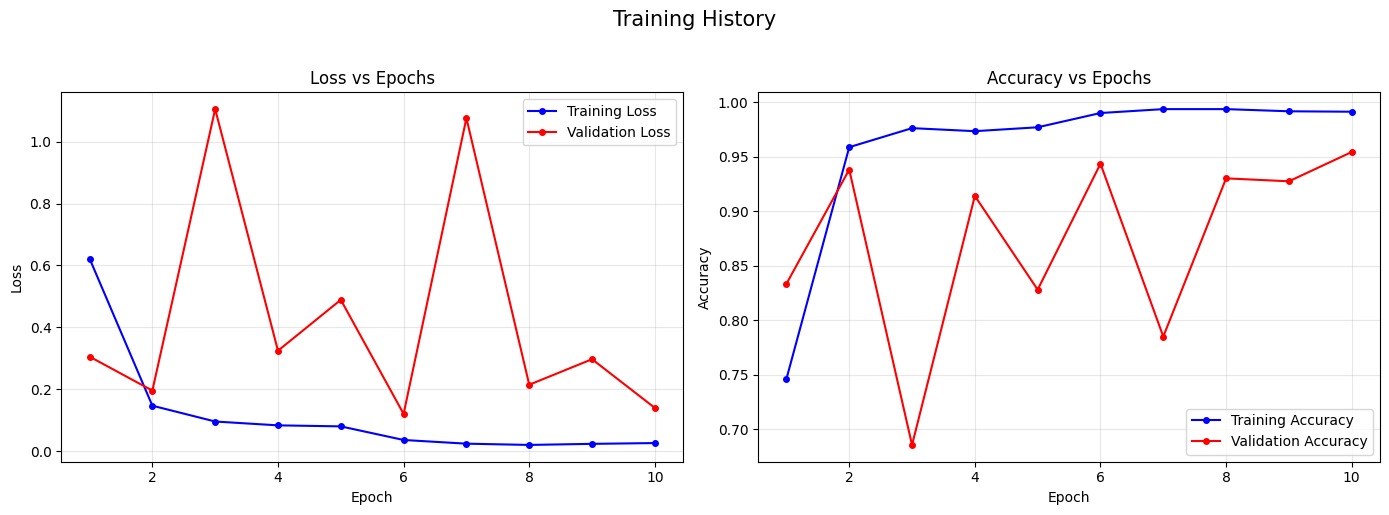
\includegraphics[width=0.95\textwidth]{images/training_history.png}
    \caption{Training and validation loss (left) and accuracy (right) over 10 epochs.}
    \label{fig:history}
\end{figure}

\subsection{Evaluation on the Standard Test Set}
On the held-out RPS test set (372 images), the final model achieved an overall accuracy of \textbf{95\%}. The per-class classification report is shown in Table~\ref{tab:classreport}.

\begin{table}[H]
\centering
\caption{Classification report on the standard test set}
\label{tab:classreport}
\begin{tabular}{lcccc}
\toprule
\textbf{Class} & \textbf{Precision} & \textbf{Recall} & \textbf{F1-score} & \textbf{Support} \\
\midrule
paper     & 1.00 & 0.86 & 0.93 & 124 \\
rock      & 0.95 & 1.00 & 0.97 & 124 \\
scissors  & 0.93 & 1.00 & 0.96 & 124 \\
\midrule
Accuracy       & \multicolumn{3}{c}{0.95} & 372 \\
Macro avg      & 0.96 & 0.95 & 0.95 & 372 \\
Weighted avg   & 0.96 & 0.95 & 0.95 & 372 \\
\bottomrule
\end{tabular}
\end{table}

\begin{figure}[H]
    \centering
    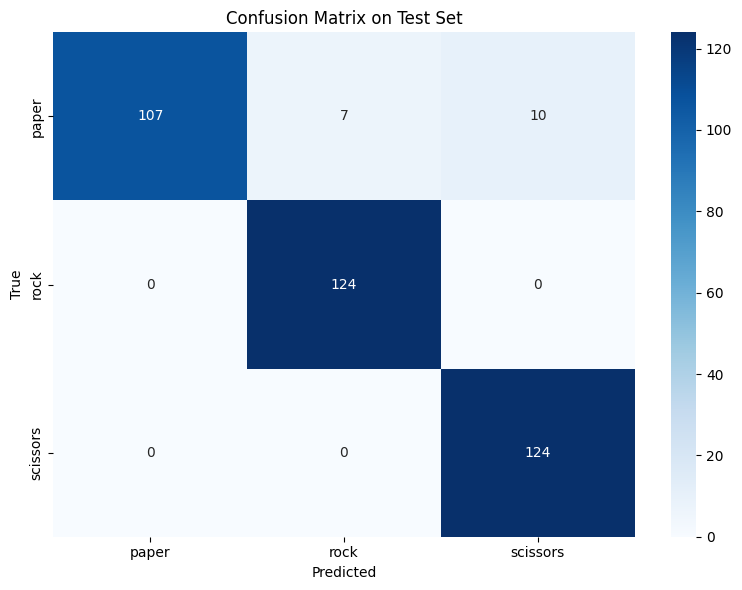
\includegraphics[width=0.65\textwidth]{images/confusion_matrix.png}
    \caption{Confusion matrix on the standard RPS test set. \texttt{rock} and \texttt{scissors} were classified perfectly; the majority of errors (17 total) came from \texttt{paper} images being confused with \texttt{rock} or \texttt{scissors}.}
    \label{fig:confmat}
\end{figure}

The confusion matrix confirms that \texttt{rock} (124/124) and \texttt{scissors} (124/124) were classified with 100\% recall, while \texttt{paper} was the weakest class (107/124 correct, recall 0.86), being confused most often with \texttt{scissors} (10 images) and occasionally with \texttt{rock} (7 images).

\subsection{Visual Error Analysis}
Out of 372 test images, 17 were misclassified. Three randomly sampled misclassified examples are shown in Figure~\ref{fig:errors}; all three happen to be \texttt{paper} images that were confused with \texttt{scissors} or \texttt{rock}, consistent with the confusion matrix above. Visually, these particular hand poses show the fingers close together or partially curled, which likely makes the rendered silhouette ambiguous between an open \texttt{paper} hand and a partially-closed \texttt{scissors}/\texttt{rock} hand.

\begin{figure}[H]
    \centering
    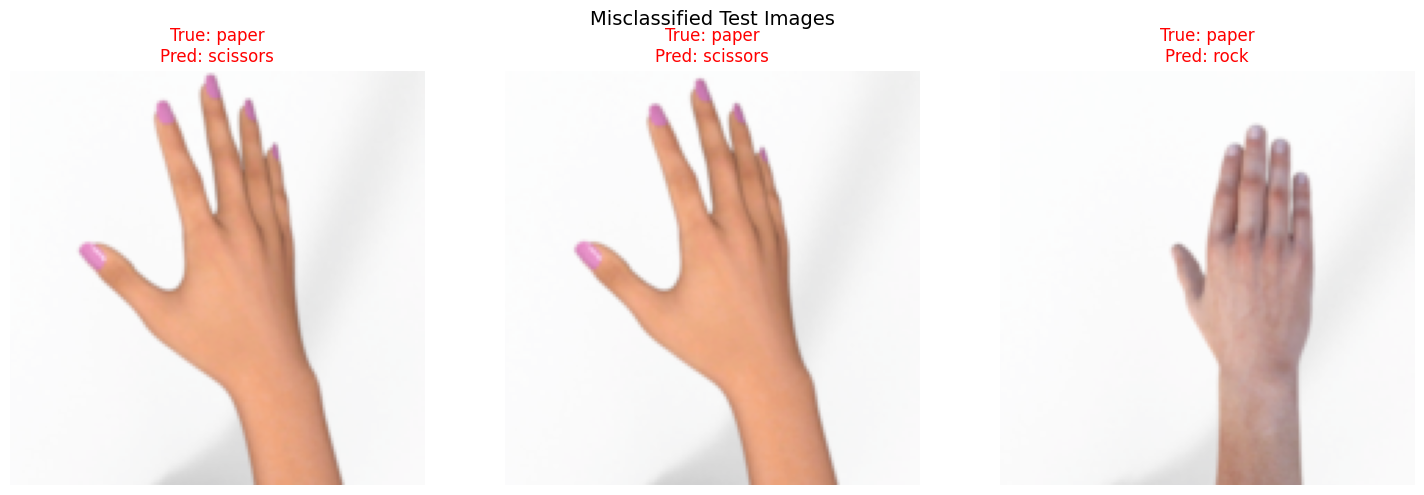
\includegraphics[width=0.95\textwidth]{images/misclassified_images.png}
    \caption{Three randomly selected misclassified test images with true vs. predicted labels.}
    \label{fig:errors}
\end{figure}

\subsection{Real-World Prediction on Custom Phone Images}
The trained model was applied to the 10 custom smartphone photographs of the author's hand. Table~\ref{tab:custom} lists the prediction and confidence for every image, and Figure~\ref{fig:custom} shows the full prediction gallery (green title = correct, red title = incorrect).

\begin{table}[H]
\centering
\caption{Model predictions on the 10 custom phone images}
\label{tab:custom}
\begin{tabular}{llccc}
\toprule
\textbf{Filename} & \textbf{True Label} & \textbf{Predicted} & \textbf{Confidence} & \textbf{Correct?} \\
\midrule
paper\_1.jpeg    & paper    & rock & 99.9\%  & No \\
paper\_2.jpeg    & paper    & rock & 100.0\% & No \\
paper\_3.jpeg    & paper    & rock & 97.6\%  & No \\
rock\_1.jpeg     & rock     & rock & 100.0\% & Yes \\
rock\_2.jpeg     & rock     & rock & 100.0\% & Yes \\
rock\_3.jpeg     & rock     & rock & 100.0\% & Yes \\
rock\_4.jpeg     & rock     & rock & 100.0\% & Yes \\
scissors\_1.jpeg & scissors & rock & 100.0\% & No \\
scissors\_2.jpeg & scissors & rock & 100.0\% & No \\
scissors\_3.jpeg & scissors & rock & 100.0\% & No \\
\bottomrule
\end{tabular}
\end{table}

\begin{figure}[H]
    \centering
    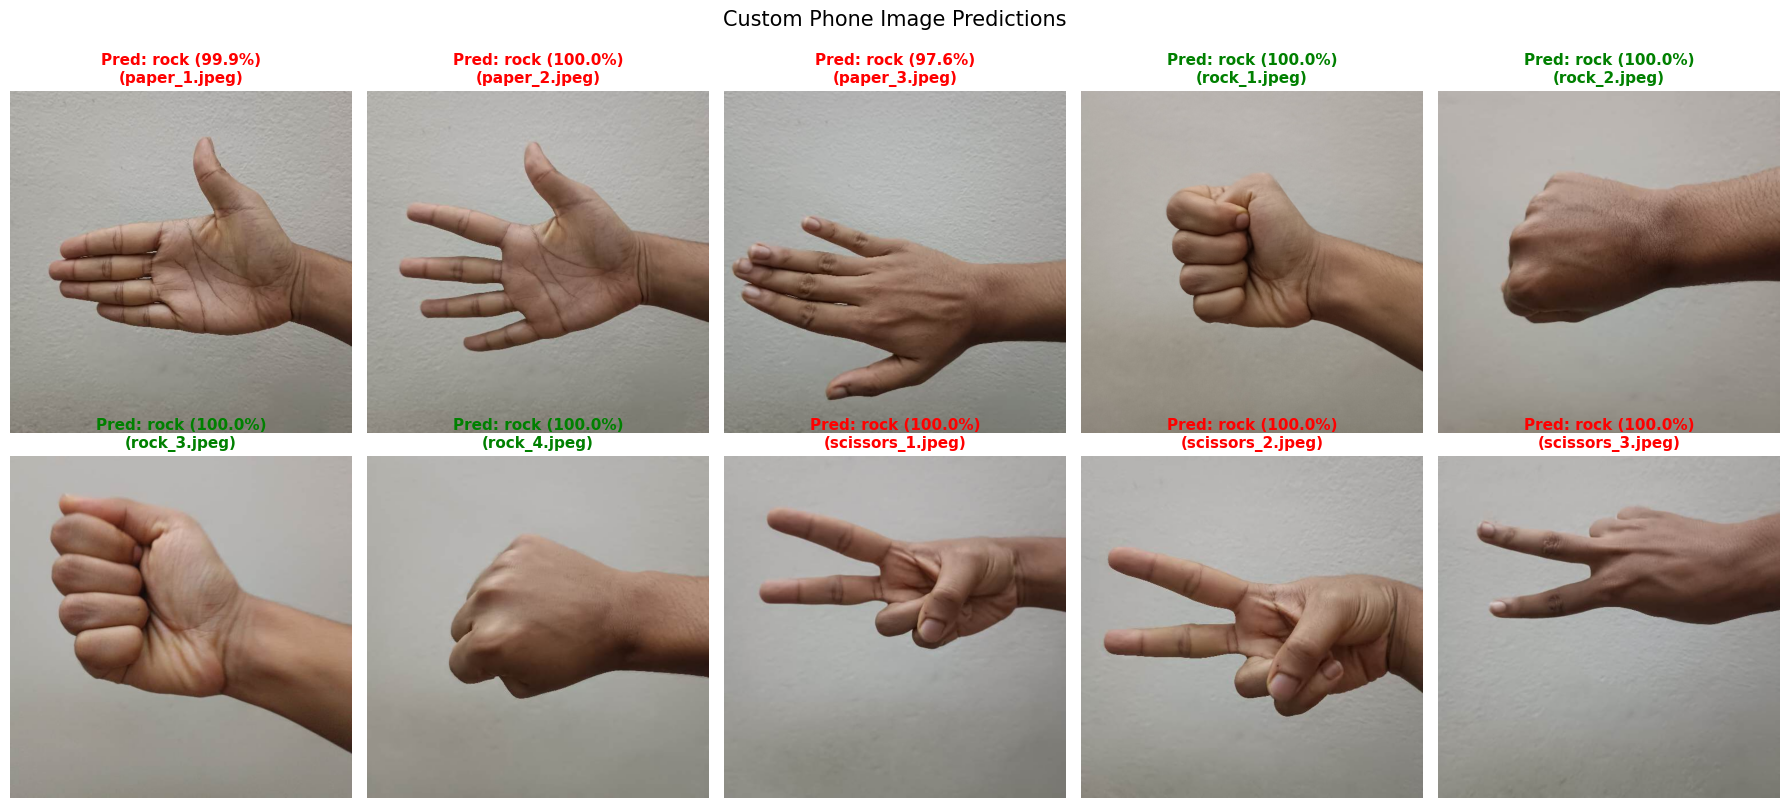
\includegraphics[width=0.95\textwidth]{images/custom_predictions_grid.png}
    \caption{Predictions on all 10 custom smartphone photographs, with predicted class and confidence percentage. Green titles indicate a correct prediction; red titles indicate an incorrect one.}
    \label{fig:custom}
\end{figure}

On the custom images, the model reached only \textbf{4/10 (40\%) accuracy}, correctly identifying every \texttt{rock} image but classifying \emph{every single} \texttt{paper} and \texttt{scissors} image as \texttt{rock} as well, almost always with near-100\% confidence. This is discussed further in Section~\ref{sec:discussion}.

% ==================================================
% 5. DISCUSSION
% ==================================================
\section{Discussion}
\label{sec:discussion}

\subsection{Performance on the Standard Dataset}
The CNN generalizes well within the distribution it was trained on: 95\% test accuracy after only 10 epochs, with \texttt{rock} and \texttt{scissors} classified perfectly and \texttt{paper} being the primary source of confusion. This is consistent with the visual similarity between an open \texttt{paper} hand at certain angles and a \texttt{scissors}/\texttt{rock} hand -- the standard RPS dataset already contains this kind of pose ambiguity across classes.

\subsection{Domain Gap on Real-World Photos}
The sharp drop in accuracy on the custom phone photographs (95\% $\to$ 40\%), and the fact that the model collapsed to predicting \texttt{rock} for almost every image regardless of the true gesture, is a textbook example of \textbf{domain shift / distribution shift}. Several concrete differences between the two image domains likely explain this:

\begin{itemize}[leftmargin=1.3cm]
    \item \textbf{Background:} The standard RPS dataset uses CGI-rendered hands on a nearly uniform, plain grey/white backdrop (Figure~\ref{fig:sample_training}), whereas the custom photos were taken against a real wall with natural shadows, texture, and lighting variation.
    \item \textbf{Hand appearance:} The training images are synthetic 3D renders with smooth, stylized skin, while the phone photos show a real human hand with skin texture, veins, and natural imperfections -- a significant appearance gap for a model trained from scratch with no pretrained features.
    \item \textbf{Framing/pose:} The RPS dataset frames the hand centrally at a fairly consistent distance and rotation range ($\pm10^{\circ}$ augmentation), while phone photos vary more in distance, angle, and where the hand sits in the frame.
    \item \textbf{Small, non-pretrained backbone:} Training a randomly initialized 619K-parameter CNN from scratch on only 2,520 images encourages the network to latch onto low-level, dataset-specific cues (background texture, rendering artifacts) rather than robust, semantic hand-shape features that would transfer to real photographs.
\end{itemize}

Interestingly, the model still correctly recognized all 4 \texttt{rock} photos. A closed fist is a visually simple, compact, high-contrast shape that seems to have been easier for the network to recognize even outside the training distribution, whereas the more detailed finger configurations of \texttt{paper} and \texttt{scissors} were not.

\subsection{Possible Improvements}
\begin{itemize}[leftmargin=1.3cm]
    \item \textbf{Transfer learning:} Initialize the convolutional backbone from a pretrained network (e.g., ResNet18/MobileNet on ImageNet) so the model relies on more general, transferable visual features instead of dataset-specific cues.
    \item \textbf{Stronger/more realistic augmentation:} Add background replacement, random cropping, and stronger color/lighting jitter during training so the model is less reliant on the plain synthetic background.
    \item \textbf{Domain adaptation / fine-tuning:} Fine-tune on a small number of real photographs (even a handful per class) to adapt the decision boundary to the real-world domain.
    \item \textbf{More diverse real training data:} Incorporate a real-photo RPS dataset (rather than only the CGI-rendered one) so the training distribution better matches the deployment distribution.
\end{itemize}

% ==================================================
% 6. REPOSITORY & REPRODUCIBILITY
% ==================================================
\section{Repository Structure and Reproducibility}

The complete project (code, custom images, and trained weights) is hosted on GitHub, following the structure required by the assignment:

\begin{lstlisting}[language=, basicstyle=\ttfamily\small, frame=single, backgroundcolor=\color{codebg}]
Lab Final/
|-- dataset/                 10 custom smartphone photos
|   |-- paper_1.jpeg .. paper_3.jpeg
|   |-- rock_1.jpeg .. rock_4.jpeg
|   |-- scissors_1.jpeg .. scissors_3.jpeg
|-- model/
|   |-- 220121.pth           Saved model state dictionary
|-- 220121.ipynb             Main Colab notebook
|-- requirements.txt
|-- .gitignore
|-- README.md
\end{lstlisting}

Running the notebook end-to-end (Runtime $\to$ Run all) automatically clones the repository, downloads the RPS dataset, trains the model, saves the weights, and reproduces every figure and table in this report -- no manual file uploads or path edits are required.

\begin{itemize}[leftmargin=1.3cm]
    \item \textbf{GitHub Repository:} \url{https://github.com/Marwanthe0/CSE/tree/main/Third\%20Year/3-2/Artificial\%20Intelligence\%20and\%20ML/Lab\%20Final}
    \item \textbf{Colab Notebook:} \url{https://colab.research.google.com/drive/1lCTyW3xMkFSMuc5Su9Zgi0NG4J7OAbLm?usp=sharing}
\end{itemize}

% ==================================================
% 7. CONCLUSION
% ==================================================
\section{Conclusion}

A three-block CNN was successfully implemented, trained, and evaluated in PyTorch for Rock--Paper--Scissors hand gesture classification, achieving \textbf{95\% accuracy} on the standard held-out test set after just 10 epochs. The full pipeline -- automated dataset retrieval, preprocessing, training, evaluation, and real-world inference -- runs end-to-end in Google Colab with a single ``Run all,'' satisfying the assignment's reproducibility requirements.

However, evaluating the model on 10 real smartphone photographs revealed a substantial \textbf{domain gap}: accuracy dropped to 40\%, with the model defaulting to the \texttt{rock} prediction for nearly every real image. This highlights an important, general lesson in applied deep learning -- strong performance on a benchmark test set (drawn from the same distribution as the training data) does not guarantee robustness to real-world deployment conditions. Bridging this gap would require techniques such as transfer learning, domain-realistic augmentation, or fine-tuning on real photographs, as discussed in Section~\ref{sec:discussion}.

\end{document}
